%%%%%%%%%%%%%%%%%%%%%%%%%%%%%%%%%%%%%%%%%
% Appendix
% 
% $Date$
% $Rev$:
% $Author$

\newpage
\appendix

% \chapter*{Appendix}\label{appendix}
\phantomsection
\addtocontents{toc}{\protect\pagebreak}
\addcontentsline{toc}{chapter}{Appendix}\hypertarget{hypertarget:appendix}{}
\addtocontents{toc}{\protect\setcounter{tocdepth}{0}}

\chapter{Wrapper Scripts}\label{appendix:wrapperScripts}
The \dir{bin/} directory of \Kieker's binary release contains some \file{.sh}  and %
\file{.bat} scripts to invoke tools included in \file{\mainJar{}}. %
The following sections give a short description of their functionality and %
list their usage outputs as printed to the standard output stream when %
called without command-line parameters. %
In addition to the standard output stream, the file \file{kieker.log} %
is used for logging output during execution.

% generated by the script gen-bin-usage-tex.sh with manual adjustments

\

\WARNBOX{%
The Windows \file{.bat} wrapper scripts must be executed from within %
the \dir{bin/} directory.
}

\section{Script \file{convertLoggingTimestamp.sh|bat}}

The script converts \KiekerMonitoringPart{} logging timestamps, %
representing the number of nanoseconds since 1~Jan 1970 00:00 UTC, to a %
human-readable textual representation in the UTC and local timezones. %

\

\noindent Main-class: {\small \class{kieker.tools.loggingTimestampConverter.LoggingTimestampConverterTool}}

\paragraph*{Usage}\

\setTextListing
\lstinputlisting[caption=]{Appendix-usage-convertLoggingTimestamp.sh.inc}

\paragraph*{Example}\

The following listing shows the command to convert two logging timestamps as %
well as the resulting output.

\enlargethispage{0.7cm}

\setTextListing
\begin{lstlisting}[caption=Execution under UNIX-like systems]
$\lstshellprompt{}$ $\textbf{bin/convertLoggingTimestamp.sh}$ $\textbf{-\,-timestamps}$ 1283156545581511026 1283156546127117246 
1283156545581511026: Mo, 30 Aug 2010 08:22:25 +0000 (UTC) (Mo, 30 Aug 2010 10:22:25 +0200 (local time))
1283156546127117246: Mo, 30 Aug 2010 08:22:26 +0000 (UTC) (Mo, 30 Aug 2010 10:22:26 +0200 (local time))
\end{lstlisting}

\begin{lstlisting}[caption=Execution under Windows]
$\lstshellprompt{}$ $\textbf{convertLoggingTimestamp.bat}$ $\textbf{-\,-timestamps}$ 1283156545581511026 1283156546127117246 
1283156545581511026: Mo, 30 Aug 2010 08:22:25 +0000 (UTC) (Mo, 30 Aug 2010 10:22:25 +0200 (local time))
1283156546127117246: Mo, 30 Aug 2010 08:22:26 +0000 (UTC) (Mo, 30 Aug 2010 10:22:26 +0200 (local time))
\end{lstlisting}

% \pagebreak

\section{Script \file{logReplay.sh|bat}}

Replays filesystem monitoring logs created by \KiekerMonitoringPart{}. %
Example applications are:
\begin{compactitem}
\item Merging multiple directories containing monitoring data into a single %
output directory. 
\item Importing a filesystem monitoring log to another monitoring log, e.g., %
a database. Therefore, an appropriate \KiekerMonitoringPart{} configuration %
file must be passed to the script (see Section~\ref{sec:monitoring:configuration}).
\item Replaying a recorded filesystem monitoring log in real-time (or faster/slower) in order to simulate %
incoming monitoring data from a running system, e.g., via JMS~(see also Appendix~\ref{appendix:usingJMS}). 
\end{compactitem}

\

\noindent Main-class: {\small \class{kieker.tools.logReplayer.FilesystemLogReplayerStarter}}

\paragraph*{Usage}\

\setTextListing
\lstinputlisting[caption=]{Appendix-usage-logReplay.sh.inc}

\paragraph*{Example}\

\noindent The following command replays the monitoring testdata included in %
the binary release to another directory:

% \pagebreak

\setTextListing
\begin{lstlisting}[caption=Execution under UNIX-like systems]
$\lstshellprompt{}$ $\textbf{bin/logReplay.sh}$
  $\textbf{-\,-inputdirs}$ $\distributedTestdataReleaseDirDistro$ 
  $\textbf{-\,-keep-logging-timestamps}$ $true$ 
  $\textbf{-\,-realtime}$ $false$
\end{lstlisting}
\begin{lstlisting}[caption=Execution under Windows]
$\lstshellprompt{}$ $\textbf{logReplay.bat}$
  $\textbf{-\,-inputdirs}$ $\distributedTestdataReleaseDirDistroWin$ 
  $\textbf{-\,-keep-logging-timestamps}$ $true$ 
  $\textbf{-\,-realtime}$ $false$
\end{lstlisting}


\section{Script \file{kax-run.sh|bat}}\label{appendix:wrapperScripts:kaxRun}

Executes a \KiekerAnalysisPart{} pipe-and-filter configuration file (\file{.kax} file), %
described in Section~\ref{sec:analysis:controller}. %

\noindent Main-class: {\small \class{kieker.tools.KaxRun}}

\paragraph*{Usage}\

\setTextListing
\lstinputlisting[caption=]{Appendix-usage-kax-run.sh.inc}

\section{Script \file{kax-viz.sh|bat}}\label{appendix:wrapperScripts:kaxViz}

Visualizes a \KiekerAnalysisPart{} pipe-and-filter configuration file (\file{.kax} file), %
described in Section~\ref{sec:analysis:controller}. %

\noindent Main-class: {\small \class{kieker.tools.KaxViz}}

\paragraph*{Usage}\

\setTextListing
\lstinputlisting[caption=]{Appendix-usage-kax-viz.sh.inc}

\section{Script \file{trace-analysis.sh|bat}}\label{appendix:wrapperScripts:traceAnalysis}

Calls \KiekerTraceAnalysis{} to analyze and visualize monitored trace data, %
as described in Chapter~\ref{chap:aspectJ}.

\

\noindent Main-class: {\small \class{kieker.tools.traceAnalysis.TraceAnalysisTool}}

% \pagebreak

\paragraph*{Usage}\

\enlargethispage{1cm}

\setTextListing
\lstinputlisting[caption=]{Appendix-usage-trace-analysis.sh.inc}

\paragraph*{Example}\

\noindent The following commands generate a deployment-level operation dependency 
graph and convert it to pdf format:

\enlargethispage{1cm}

\setTextListing
\begin{lstlisting}[caption=Execution under UNIX-like systems]
$\lstshellprompt{}$ $\textbf{bin/trace-analysis.sh}$
  $\textbf{-\,-inputdirs}$ $\distributedTestdataReleaseDirDistro$ 
  $\textbf{-\,-outputdir}$ . 
  $\textbf{-\,-plot-Deployment-Operation-Dependency-Graph}$
$\lstshellprompt{}$ $\textbf{dot}$ $\textbf{-T}$ pdf  deploymentOperationDependencyGraph.dot > deploymentOperationDependencyGraph.pdf
\end{lstlisting}

\begin{lstlisting}[caption=Execution under Windows]
$\lstshellprompt{}$ $\textbf{trace-analysis.bat}$
  $\textbf{-\,-inputdirs}$ $\distributedTestdataReleaseDirDistroWin$ 
  $\textbf{-\,-outputdir}$ . 
  $\textbf{-\,-plot-Deployment-Operation-Dependency-Graph}$
$\lstshellprompt{}$ $\textbf{dot}$ $\textbf{-T}$ pdf  deploymentOperationDependencyGraph.dot > deploymentOperationDependencyGraph.pdf
\end{lstlisting}

\noindent Additional examples can be found in Chapter~\ref{chap:aspectJ}.

\section{Script \file{dotPic-fileConverter.sh|bat}}\label{appendix:wrapperScripts:dotPicFileConverter}

Converts each \file{.dot} and \file{.pic} file, e.g., diagrams generated by %
\KiekerTraceAnalysis{} (Section~\ref{chap:aspectJ}), located in a directory %
into desired graphic output formats. %
This scripts simply calls the \textit{Graphviz} and \textit{PlotUtils} tools \file{dot} and \file{pic2plot}.

\paragraph*{Usage}\

\setTextListing
\lstinputlisting[caption=,firstline=3,lastline=3]{Appendix-usage-dotPic-fileConverter.sh.inc}

\paragraph*{Example}\

\noindent The following command converts each \file{.dot} and \file{.pic} file located in the %
directory \dir{out/} to files in \file{.pdf} and \file{.png} format:

\setTextListing
\begin{lstlisting}[caption=Execution under UNIX-like systems]
$\lstshellprompt{}$ $\textbf{bin/dotPic-fileConverter.sh}$ out/ pdf png
\end{lstlisting}
\begin{lstlisting}[caption=Execution under Windows]
$\lstshellprompt{}$ $\textbf{dotPic-fileConverter.bat}$ out\ pdf png
\end{lstlisting}

\chapter{Java~EE Servlet Container Example}\label{appendix:JavaEEServletExample}
Using the sample Java web application %
MyBatis JPetStore,\footnote{\url{http://www.mybatis.org/spring/sample.html}} this example %
demonstrates how to employ \KiekerMonitoringPart{} for monitoring a Java application %
running in a Java~EE container---in this case Jetty.\footnote{\url{http://www.eclipse.org/jetty/}} %
Monitoring probes based on the Java~EE Servlet API, Spring, %
and AspectJ are used to monitor execution, trace, and session data (see Section~\ref{chap:aspectJ}). %
The directory \dir{\JavaEEServletExampleReleaseDirDistro/} contains the prepared Jetty %
server with the MyBatis JPetStore application and the \Kieker-based demo %
analysis application known from \url{http://demo.kieker-monitoring.net/}. %

\section{Setting}

The subdirectory \file{jetty/} includes the %
Jetty server with the JPetStore application already deployed to the server's %
\file{webapps/} directory. The example is prepared to use two alternative %
types of \Kieker{} probes: either the \Kieker{} Spring interceptor (default) or the 
\Kieker{} AspectJ aspects. Both alternatives additionally use \Kieker{}'s Servlet 
filter. %

\paragraph{Required Libraries and \KiekerMonitoringPart{} Configuration}

Both settings require the files \file{\aspectJWeaverJar{}} and \file{\mainJar}, %
which are already included in the webapps's \dir{WEB-INF/lib/} directory. %
Also, a \Kieker{} configuration file is already included in the Jetty's root directory, %
where it is considered for configuration by \KiekerMonitoringPart{} in both modes. 

\paragraph{Servlet Filter (Default)}

The file \file{web.xml} is located in the webapps's %
\dir{WEB-INF/} directory. \Kieker{}'s Servlet filters are already enabled: 

\setXMLListing
\lstinputlisting[firstline=50,lastline=61, numbers=none, linewidth=1\textwidth, caption=Enabling the Servlet filter in \file{web.xml}]{\JavaEEServletExampleDir/jetty/webapps/jpetstore/WEB-INF/web.xml}

\noindent This filter can be used with both the Spring-based and the %
AspectJ-based instrumentation mode.

\paragraph{Spring-based Instrumentation (Default)}

\Kieker{}'s Spring interceptor are already enabled in the file 
\file{applicationContext.xml}, located in the webapps's \dir{WEB-INF/} directory: 

\setXMLListing
\lstinputlisting[firstline=38,lastline=43, numbers=none, linewidth=1\textwidth, caption=Enabling the Spring interceptor in \file{applicationContext.xml}]{\JavaEEServletExampleDir/jetty/webapps/jpetstore/WEB-INF/applicationContext.xml}

\NOTIFYBOX{When using, for example, the \texttt{@Autowired} feature in your Spring beans, it can be necessary to force the usage of CGLIB proxy objects with \texttt{<aop:aspectj-autoproxy proxy-target-class="true"/>}.}

\paragraph{AspectJ-based Instrumentation}

\enlargethispage{1cm}

In order to use AspectJ-based instrumentation, the following changes need to 
be performed. The file \file{start.ini}, located in Jetty's root directory, %
allows to pass various JVM arguments, JVM system properties, and other options %
to the server on startup. When using AspectJ for instrumentation, the respective %
JVM argument needs to be activated in this file. %

The AspectJ configuration file \file{aop.xml} is already located in the %
webapps's\linebreak \dir{WEB-INF/classes/META-INF/} directory and configured to instrument %
the JPetStore classes with \Kieker{}'s \class{OperationExecutionAspectFull} aspect %
(Section~\ref{chap:aspectJ}). 

\

When using the AspectJ-based instrumentation, make sure to disable the Spring %
interceptor in the file \file{applicationContext.xml}, mentioned above. %

\begin{compactenum}
\item Start the Jetty server using the \file{start.jar} file (e.g., via \texttt{java -jar start.jar}). You should make %
   sure that the server started properly by taking a look at %
   the console output that appears during server startup.  
\item Now, you can access the JPetStore application by opening the URL
   \url{http://localhost:8080/jpetstore/} (Figure~\ref{fig:jpetstore}). %
   \Kieker{} initialization messages should appear in the console output. %
   
\begin{figure}[h]\centering
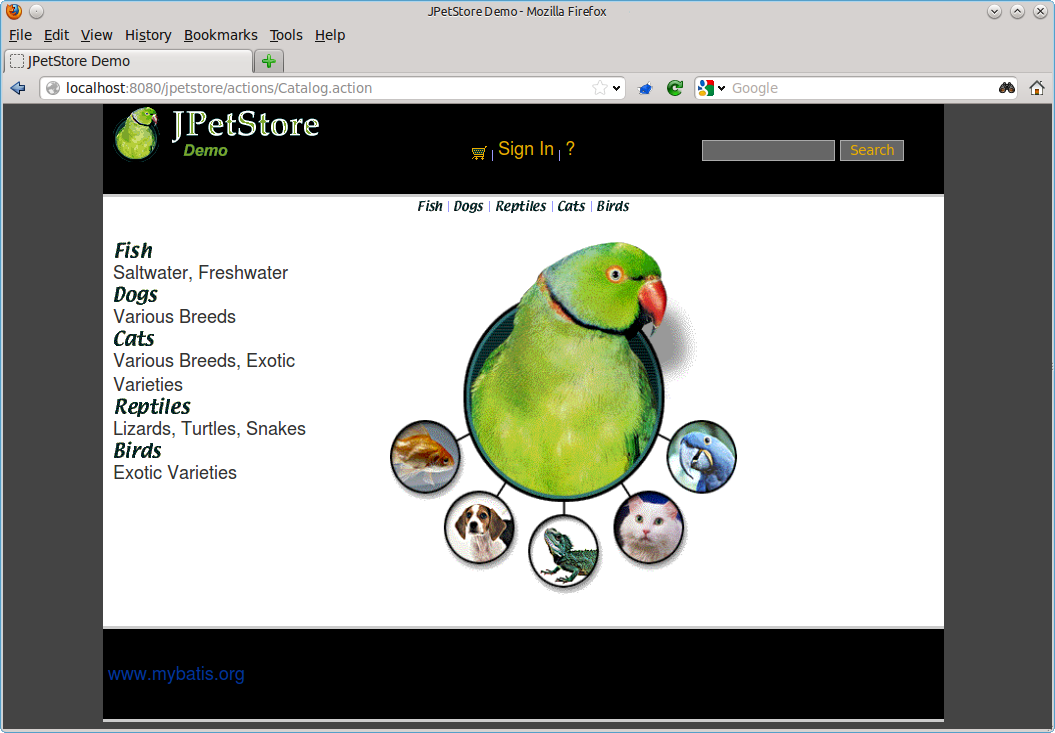
\includegraphics[width=0.8\textwidth]{images/jpetstore-example-FFscrsh}
\caption{MyBatis JPetStore}\label{fig:jpetstore}%
\end{figure}
   
\item   Browse through the application to generate some monitoring data. %
\item In this example, \Kieker{} is configured to write the monitoring data %
      to JMX in order to communicate with the \Kieker-based demo analysis %
      application, which is accessible via \url{localhost:8080/livedemo/}.
   
\item In order to write the monitoring data to the file system, the %
      JMX writer needs to be disabled in the file \file{kieker.monitoring.properties}, %
      which is located in the directory \file{webapps/jpetstore/WEB-INF/classes/META-INF/}.
      After a restart of the Jetty server, the Kieker startup output includes the %
      information where the monitoring data is written to (should be a %
      \dir{kieker-<DATE-TIME>/} directory) located in the default temporary %
      directory. %
   This data can be analyzed and visualized using \KiekerTraceAnalysis{}, %
   as described in Chapter~\ref{chap:aspectJ}.
\end{compactenum}

\medskip

 

\chapter{Using the JMS Writer and Reader}\label{appendix:usingJMS}
This chapter gives a brief description on how to use the \class{AsyncJmsWriter} and \class{JmsReader} %
classes. The directory \dir{\JMSBookstoreApplicationReleaseDirDistro/} contains the %
sources, gradle scripts etc.\ used in this example. It is based on the Bookstore %
application with manual instrumentation presented in Chapter~\ref{chap:example}. %

The following sections provide step-by-step instructions for the %
ActiveMQ JMS server implementation (Section~\ref{example:jms:activemq}).
The general procedure for this example is the following:

\medskip

\begin{compactenum}
 \item Download and prepare the respective JMS server implementation
 \item Copy required libraries to the example directory
 \item Start the JMS server
 \item Start the analysis instance which receives records via JMS
 \item Start the monitoring instance which sends records via JMS
\end{compactenum}

\

\WARNBOX{\quad\\Due to a bug in some JMS servers, avoid paths including white spaces.}

\section{ActiveMQ}\label{example:jms:activemq}

\subsection{Download and Prepare ActiveMQ}

Download an ActiveMQ archive from \url{http://activemq.apache.org/download.html}
and decompress it to the base directory of the example. Note, that there are two different %
distributions, one for Unix/Linux/Cygwin and another one for Windows, and that the latest supported version of ActiveMQ compatible with Java 7 is 5.14.5. 

Under \UnixLikeSystems{}, you'll need to set the executable-bit of the start script:

\setBashListing
\begin{lstlisting}[caption=]
 #\lstshellprompt{}# chmod +x bin/activemq
\end{lstlisting}

\noindent Also under \UnixLikeSystems{}, make sure that the file \file{bin/activemq} %
includes UNIX line endings (e.g., using your favorite editor or the \textit{dos2unix} tool).

\subsection{Copy ActiveMQ Libraries}

Copy the following files from the ActiveMQ release to the %
\dir{lib/} directory of this example:

\medskip

\enlargethispage{0.5cm}

\begin{compactenum}
\item \file{activemq-all-<version>.jar} (from ActiveMQ's base directory)
\item \file{slf4j-log4j<version>.jar} (from ActiveMQ's \dir{lib/optional} directory)
\item \file{log4j-<version>.jar} (from ActiveMQ's \dir{lib/optional} directory)
\end{compactenum}

\subsection{Kieker Monitoring Configuration for ActiveMQ}

The file \file{src-resources/META-INF/kieker.\-monitoring.\-pro\-perties-activeMQ} %
is already configured to use the \class{JmsWriter} via ActiveMQ. The important properties are %
the definition of the provider URL and the context factory:

\setPropertiesListing
\lstinputlisting[firstline=12,lastline=12,caption=Excerpt from \file{kieker.monitoring.properties-activemq} configuring the provider URL of the JMS writer via ActiveMQ]{\JMSBookstoreApplicationDir/src-resources/META-INF/kieker.monitoring.properties-activemq}

\setPropertiesListing
\lstinputlisting[firstline=21,lastline=21,caption=Excerpt from \file{kieker.monitoring.properties-activemq} configuring the context factory of the JMS writer via ActiveMQ]{\JMSBookstoreApplicationDir/src-resources/META-INF/kieker.monitoring.properties-activemq}

\subsection{Running the Example}

% \paragraph*{Execution}%
 The execution of the example is performed by the following three steps:
\begin{enumerate}
\item Start the JMS server (you may have to set your \class{JAVA\_HOME} variable first):

\setBashListing
\begin{lstlisting}[caption=Start of the JMS server under UNIX-like systems]
#\lstshellprompt{}# bin/activemq start
\end{lstlisting}
\begin{lstlisting}[caption=Start of the JMS server under Windows]
#\lstshellprompt{}# bin\#activemq start
\end{lstlisting}
\item Start the analysis part (in a new terminal):
\setBashListing
\begin{lstlisting}[caption=Start the analysis part under UNIX-like systems]
#\lstshellprompt{}# ./gradlew runAnalysisActiveMQ
\end{lstlisting}
\begin{lstlisting}[caption=Start the analysis part under Windows]
#\lstshellprompt{}# gradlew.bat runAnalysisActiveMQ
\end{lstlisting}
\item Start the instrumented Bookstore (in a new terminal):
\setBashListing
\begin{lstlisting}[caption=Start the analysis part under UNIX-like systems]
#\lstshellprompt{}# ./gradlew runMonitoringActiveMQ
\end{lstlisting}
\begin{lstlisting}[caption=Start the analysis part under Windows]
#\lstshellprompt{}# gradlew.bat runMonitoringActiveMQ
\end{lstlisting}
\end{enumerate}


\chapter{Using the AMQP Writer and Reader}\label{appendix:usingAMQP}
This chapter gives a brief description on how to use the \class{AmqpWriter} and \class{AmqpReader} %
classes, which allow to use Kieker with AMQP-based queue implementations such as %
RabbitMQ.\footnote{\url{http://www.rabbitmq.com}} The directory \dir{\AMQPBookstoreApplicationReleaseDirDistro/} %
contains the sources, gradle scripts etc.\ used in this example. It is based on the Bookstore %
application with manual instrumentation presented in Chapter~\ref{chap:example}. %

The following paragraphs provide step-by-step instructions for the popular AMQP implementation RabbitMQ.%

\section{Preparation}

\subsection{Download and Install RabbitMQ}
Download the RabbitMQ distribution from \url{http://www.rabbitmq.com/download.html} and follow the installation %
instructions for your OS. Since RabbitMQ requires Erlang, additional software packages may have to be installed %
on your machine.
\par In order to use RabbitMQ's integrated management UI, you may have to enable the appropriate plugin first. This is %
done by issuing the following command from the command line. 

\setBashListing
\begin{lstlisting}[caption=Enable the management UI under UNIX-like systems]
#\lstshellprompt{}# rabbitmq-plugins enable rabbitmq_management
\end{lstlisting}
\begin{lstlisting}[caption=Enable the management UI under Windows]
#\lstshellprompt{}# rabbitmq-plugins enable rabbitmq_management
\end{lstlisting}

Once the UI is enabled, you may access it at port 15672 by default. %

\subsection{Configure RabbitMQ}
Once the RabbitMQ server is installed and started, create a queue for Kieker to use. This can be done easily using %
RabbitMQ's management UI. It is accessible via \url{http://localhost:15672} (the default credentials are \texttt{guest:guest}) We will assume a queue named \parameterValue{kieker} for the remainder of this %
example. Please note the following caveats when configuring the server:

\begin{compactenum}
 \item If you choose to create a transient queue, the entire queue (not just the queued messages) is destroyed %
 on server shutdown and must be re-created manually. %
 \item The RabbitMQ server's default permissions grant access only from \hostname{localhost}. If your RabbitMQ server runs %
 on a remote machine, you have to set the permissions accordingly. %
\end{compactenum}

\subsection{Kieker Monitoring Configuration for RabbitMQ}
The file \file{src-resources/META-INF/kieker.\-monitoring.\-pro\-perties} %
is already configured to use the \class{AMQPWriter}. The important properties are %
the server URI and the queue name. %

\setPropertiesListing
\lstinputlisting[firstline=9,lastline=9,caption=Excerpt from \file{kieker.monitoring.properties} configuring the URI of the AMQP server]{\AMQPBookstoreApplicationDir/src-resources/META-INF/kieker.monitoring.properties}

\setPropertiesListing
\lstinputlisting[firstline=15,lastline=15,caption=Excerpt from \file{kieker.monitoring.properties} configuring the AMQP queue name]{\AMQPBookstoreApplicationDir/src-resources/META-INF/kieker.monitoring.properties}

\section{Running the Example}
The execution of the example is performed by the following three steps:
\begin{enumerate}
\item Ensure that the RabbitMQ server is started and the configured queue is accessible.

\item Start the analysis part (in a new terminal):
\setBashListing
\begin{lstlisting}[caption=Start the analysis part under UNIX-like systems]
#\lstshellprompt{}# ./gradlew runAnalysisAMQP
\end{lstlisting}
\begin{lstlisting}[caption=Start the analysis part under Windows]
#\lstshellprompt{}# gradlew.bat runAnalysisAMQP
\end{lstlisting}
\item Start the instrumented Bookstore (in a new terminal):
\setBashListing
\begin{lstlisting}[caption=Start the analysis part under UNIX-like systems]
#\lstshellprompt{}# ./gradlew runMonitoringAMQP
\end{lstlisting}
\begin{lstlisting}[caption=Start the analysis part under Windows]
#\lstshellprompt{}# gradlew.bat runMonitoringAMQP
\end{lstlisting}
\end{enumerate}

\chapter{Sigar-Based Samplers for System-Level Monitoring}\label{appendix:SigarBasedSamplers}
This chapter gives a brief description on how to use the included %
periodic samplers (Section~\ref{sec:componentsMonitoring:monitoringController:periodicSamplers}) %
for monitoring CPU utilization and memory/swap usage. %
The directory \dir{\SigarExampleReleaseDirDistro/} contains the %
sources, gradle scripts etc.\ used in this example. %
These samplers employ the Sigar API~\cite{HypericSigarWebsite}. \\%

\section{Preparation}

\begin{compactenum}
\item Copy the files \file{\mainJarEMF} and \file{\sigarJar} from the %
binary distribution to the example's \dir{lib/} directory.
\item Additionally, depending on the underlying system platform, %
corresponding Sigar native libraries need to be placed in the example's \dir{lib/} directory. %
Kieker's \dir{lib/sigar-native-libs/} folder already includes the right libraries for 32 and 64~bit Linux/Windows platforms. %
Native libraries for other platforms can be downloaded from~\cite{HypericSigarWebsite}. %
\end{compactenum}

\section{Using the Sigar-Based Samplers}

\WARNBOX{
	Using a very short sampling period with Sigar ($< 500$ ms) can result in monitoring log entries with NaN values. 
}

The Sigar API~\cite{HypericSigarWebsite} provides access to a number of system-level inventory and monitoring data, %
e.g., regarding memory, swap, cpu, file system, and network devices. %
Kieker includes Sigar-based samplers %
for monitoring CPU utilization %
(\class{CPUsDetailedPercSampler}, \class{CPUsCombinedPercSampler}) %
and memory/swap usage (\class{MemSwapUsageSampler}). %
When registered as a periodic sampler (Section~\ref{sec:componentsMonitoring:monitoringController:periodicSamplers}), %
these samplers collect the data of interest employing the Sigar API, %
and write monitoring records of types \class{CPUUtilizationRecord}, %
\class{ResourceUtilizationRecord}, and \class{MemSwapUsageRecord} respectively %
to the configured monitoring log/stream. %

Listing~\ref{listing:sigarSamplerMonitoringStarterExample} shows an excerpt from %
this example's \class{MonitoringStarter} %
which creates and registers two Sigar-based peridioc samplers. %
For reasons of performance and thread-safety, the \class{SigarSamplerFactory} %
should be used to create instances of the Sigar-based Samplers. 

%\pagebreak

\setJavaCodeListing
\lstinputlisting[firstline=38, lastline=51, firstnumber=38, caption=Excerpt from MonitoringStarter.java, label=listing:sigarSamplerMonitoringStarterExample]{\SigarExampleDir/src/kieker/examples/userguide/appendixSigar/MonitoringStarter.java}

\noindent Based on the existing samplers, users can easily create custom Sigar-based %
samplers by extending the class \class{AbstractSigarSampler}. For example, Listing~%
\ref{listing:sigarSamplerMethod} in Section~\ref{sec:componentsMonitoring:monitoringController:periodicSamplers} %
shows the \class{MemSwapUsageSampler}'s \method{sample} method. %
Typically, it is also required to define a corresponding monitoring record type, %
as explained in Section~\ref{sec:componentsMonitoring:monitoringRecords}. %
When implementing custom Sigar-based samplers, the \class{SigarSamplerFactory}'s \method{getSigar} method should %
be used to retrieve a \class{Sigar} instance. %

This example uses a stand-alone Java application to set up %
a Sigar-based monitoring process. When using servlet containers,  %
users may consider implementing this routine as a \class{ServletContextListener}, %
which are executed when the container is started and shutdown. %
As an example, Kieker includes a \class{CPUMemUsageServletContextListener}. %

\section{Executing the Example}

The execution of the example is performed by the following two steps:\\

\begin{compactenum}
\item Monitoring CPU utilization and memory usage for 30~seconds (class \class{MonitoringStarter}):
\setBashListing
\begin{lstlisting}[caption=Start of the monitoring under UNIX-like systems]
#\lstshellprompt{}# #\textbf{./gradlew}# runMonitoring
\end{lstlisting}
\begin{lstlisting}[caption=Start of the monitoring under Windows]
#\lstshellprompt{}# #\textbf{gradlew.bat}# runMonitoring
\end{lstlisting}

Kieker's console output lists the location of the directory containing the file system %
monitoring log. The following listing shows an excerpt: %

%\enlargethispage{1.5cm}
\pagebreak
\setBashListing
\begin{lstlisting}
 Writer: 'kieker.monitoring.writer.filesystem.AsciiFileWriter'
     Configuration:
             kieker.monitoring.writer.filesystem.AsciiFileWriter.QueueFullBehavior='0'
             kieker.monitoring.writer.filesystem.AsciiFileWriter.QueueSize='10000'
             kieker.monitoring.writer.filesystem.AsciiFileWriter.customStoragePath=''
             kieker.monitoring.writer.filesystem.AsciiFileWriter.storeInJavaIoTmpdir='true'
     Writer Threads (1): 
             Finished: 'false'; Writing to Directory: '/tmp/kieker-20110511-10095928-UTC-avanhoorn-thinkpad-KIEKER-SINGLETON'
\end{lstlisting}

A sample monitoring log can be found in the directory \dir{\SigarExampleReleaseDirDistro/testdata/kieker-20110511-10095928-UTC-avanhoorn-thinkpad-KIEKER-SINGLETON/}.

\item Analyzing the monitoring data (class \class{AnalysisStarter}):

\setBashListing
\begin{lstlisting}[caption=Start of the monitoring data analysis under UNIX-like systems]
#\lstshellprompt{}# #\textbf{./gradlew}# runAnalysis #\textbf{-Danalysis.directory}#=</path/to/monitoring/log/>
\end{lstlisting}
\begin{lstlisting}[caption=Start of the monitoring data analysis under Windows]
#\lstshellprompt{}# #\textbf{gradlew.bat}# runAnalysis #\textbf{-Danalysis.directory}#=</path/to/monitoring/log/>
\end{lstlisting}

You need to replace \dir{</path/to/monitoring/log/>} by the location of the file system monitoring log. %
You can also use the above-mentioned monitoring log included in the example. %

The \class{AnalysisStarter} produces a simple console output for each monitoring record, %
as shown in the following excerpt: 

\setBashListing
\begin{lstlisting}
Wed, 11 May 2011 10:10:01 +0000 (UTC): [CPU] host: thinkpad ; cpu-id: 0 ; utilization: 0.00 %
Wed, 11 May 2011 10:10:01 +0000 (UTC): [CPU] host: thinkpad ; cpu-id: 1 ; utilization: 0.00 %
Wed, 11 May 2011 10:10:01 +0000 (UTC): [Mem/Swap] host: thinkpad ; mem usage: 722.0 MB ; swap usage: 0.0 MB
Wed, 11 May 2011 10:10:06 +0000 (UTC): [CPU] host: thinkpad ; cpu-id: 0 ; utilization: 5.35 %
Wed, 11 May 2011 10:10:06 +0000 (UTC): [CPU] host: thinkpad ; cpu-id: 1 ; utilization: 1.31 %
Wed, 11 May 2011 10:10:06 +0000 (UTC): [Mem/Swap] host: thinkpad ; mem usage: 721.0 MB ; swap usage: 0.0 MB
Wed, 11 May 2011 10:10:11 +0000 (UTC): [CPU] host: thinkpad ; cpu-id: 0 ; utilization: 1.80 %
Wed, 11 May 2011 10:10:11 +0000 (UTC): [CPU] host: thinkpad ; cpu-id: 1 ; utilization: 0.20 %
Wed, 11 May 2011 10:10:11 +0000 (UTC): [Mem/Swap] host: thinkpad ; mem usage: 721.0 MB ; swap usage: 0.0 MB
Wed, 11 May 2011 10:10:16 +0000 (UTC): [CPU] host: thinkpad ; cpu-id: 0 ; utilization: 1.40 %
Wed, 11 May 2011 10:10:16 +0000 (UTC): [CPU] host: thinkpad ; cpu-id: 1 ; utilization: 0.79 %
Wed, 11 May 2011 10:10:16 +0000 (UTC): [Mem/Swap] host: thinkpad ; mem usage: 721.0 MB ; swap usage: 0.0 MB
Wed, 11 May 2011 10:10:21 +0000 (UTC): [CPU] host: thinkpad ; cpu-id: 0 ; utilization: 1.80 %
Wed, 11 May 2011 10:10:21 +0000 (UTC): [CPU] host: thinkpad ; cpu-id: 1 ; utilization: 0.79 %
Wed, 11 May 2011 10:10:21 +0000 (UTC): [Mem/Swap] host: thinkpad ; mem usage: 721.0 MB ; swap usage: 0.0 MB
Wed, 11 May 2011 10:10:26 +0000 (UTC): [CPU] host: thinkpad ; cpu-id: 0 ; utilization: 0.40 %
Wed, 11 May 2011 10:10:26 +0000 (UTC): [CPU] host: thinkpad ; cpu-id: 1 ; utilization: 0.59 %
Wed, 11 May 2011 10:10:26 +0000 (UTC): [Mem/Swap] host: thinkpad ; mem usage: 721.0 MB ; swap usage: 0.0 MB
\end{lstlisting}


\end{compactenum}


\chapter{\KiekerMonitoringPart{} Default Configuration}\label{sec:appdx:monitoringproperties}
This is the file \file{\kiekerExampleMonitoringProperties} from the binary release and 
constitutes \KiekerMonitoringPart{}'s default configuration. %
Section~\ref{sec:monitoring:configuration} describes how to use a custom configuration.

\

\setPropertiesListing
\lstinputlisting[caption=\monitoringPropertiesFile]{../../kieker-monitoring/src-resources/META-INF/kieker.monitoring.default.properties}


\chapter{Additional Source Code Listings}\label{appendix:additionalSourceCode}
\section{MyNamedPipeManager and MyPipe}\label{appendix:pipeListings}

\enlargethispage{1cm}

      \setJavaCodeListing
      \lstinputlisting[firstline=22, firstnumber=22,caption=MyNamedPipeManager.java]{\customComponentsBookstoreApplicationDir/src/kieker/examples/userguide/ch3and4bookstore/MyNamedPipeManager.java}
\newpage
      \setJavaCodeListing
      \lstinputlisting[firstline=22, firstnumber=22, caption=MyPipe.java]{\customComponentsBookstoreApplicationDir/src/kieker/examples/userguide/ch3and4bookstore/MyPipe.java}
      
      \setJavaCodeListing
      \lstinputlisting[firstline=21, firstnumber=21, caption=PipeData.java]{\customComponentsBookstoreApplicationDir/src/kieker/examples/userguide/ch3and4bookstore/PipeData.java}

\chapter{Example Console Outputs}\label{appendix:exampleConsoleOutputs}
\section{Quick Start Example (Chapter~\ref{chap:example})}\label{sec:appendix:manualInstrumentation:output}
% \subsubsection{Monitoring}
% 		The following listing shows the produced log during a run of the Bookstore Application with the manual monitoring probes.
\setTextListing
\lstinputlisting[caption=Execution of the manually instrumented Bookstore application (Section~\ref{sec:example:monitoring})]
{ch2-quickstart-example/kieker-20130910-120352847-UTC-myHost-KIEKER-SINGLETON-monitoring.stdout}
\newpage
% \subsubsection{Analysis}
% 		The second listing is the log during the analysis of the produced data. It can be seen that some of the calls are accepted and some others refused.
\setTextListing
\lstinputlisting[caption=Execution of the example analysis (Section~\ref{sec:example:analysis})]
{ch2-quickstart-example/kieker-20130910-120352847-UTC-myHost-KIEKER-SINGLETON-analysis.stdout}
\newpage	
\section{Trace Monitoring, Analysis \& Visualization (Chapter \ref{chap:aspectJ})}%
\label{sec:appendix:exampleConsoleOutputs:aspectJExample}
\setTextListing
\begin{lstlisting}[caption=Execution of the Bookstore with AspectJ trace instrumentation (Section~\ref{sec:traceAnalysis:instr:AspectJ})]
Bookstore.main: Starting request 0
Bookstore.main: Starting request 1
Bookstore.main: Starting request 2
Bookstore.main: Starting request 3
Bookstore.main: Starting request 4
Apr 14, 2014 10:35:04 PM kieker.monitoring.core.configuration.ConfigurationFactory createSingletonConfiguration
INFO: Loading properties from properties file in classpath: 'META-INF/kieker.monitoring.properties'
Apr 14, 2014 10:35:04 PM kieker.monitoring.core.controller.MonitoringController createInstance
INFO: Current State of kieker.monitoring (1.9) Status: 'enabled'
        Name: 'KIEKER'; Hostname: 'myHost'; experimentID: '1'
JMXController: JMX disabled
RegistryController: 0 strings registered.
TimeSource: 'kieker.monitoring.timer.SystemNanoTimer'
        Time in nanoseconds (with nanoseconds precision) since Thu Jan 01 01:00:00 CET 1970'
ProbeController: disabled
WriterController:
        Number of Inserts: '0'
        Automatic assignment of logging timestamps: 'true'
Writer: 'kieker.monitoring.writer.filesystem.AsciiFileWriter'
        Configuration:
                kieker.monitoring.writer.filesystem.AsciiFileWriter.flush='true'
                kieker.monitoring.writer.filesystem.AsciiFileWriter.maxLogSize='-1'
                kieker.monitoring.writer.filesystem.AsciiFileWriter.QueueFullBehavior='0'
                kieker.monitoring.writer.filesystem.AsciiFileWriter.MaxShutdownDelay='-1'
                kieker.monitoring.writer.filesystem.AsciiFileWriter.maxEntriesInFile='25000'
                kieker.monitoring.writer.filesystem.AsciiFileWriter.bufferSize='8192'
                kieker.monitoring.writer.filesystem.AsciiFileWriter.maxLogFiles='-1'
                kieker.monitoring.writer.filesystem.AsciiFileWriter.customStoragePath=''
                kieker.monitoring.writer.filesystem.AsciiFileWriter.QueueSize='10000'
        Records lost: 0
        Writer Threads (1): 
                Finished: 'false'; Writing to Directory: '/tmp/kieker-20140414-203504785-UTC-myHost-KIEKER'
Sampling Controller: Periodic Sensor available: Poolsize: '0'; Scheduled Tasks: '0'
Apr 14, 2014 10:35:04 PM kieker.monitoring.core.registry.ControlFlowRegistry <clinit>
INFO: First threadId will be 1063271724524503040
\end{lstlisting}




% \chapter{Ant Scripts}\label{appendix:antScripts}
% \section{Quick Start Example (Chapter \ref{chap:example})}
The following \file{build.xml} and \file{build.properties} files can be %
used for compiling and executing the manually instrumentated Bookstore %
application and the analysis, as described in Chapter~\ref{chap:example}. %
The files are included in the directory \file{\manualInstrumentedBookstoreApplicationDirDistro{}/}.

      In order to run the analysis of the application, it is necessary to pass the location of the monitoring log directory. This is done via the parameter \textit{analysis.directory}, e.g.:
      \setBashListing
      \begin{lstlisting}[caption=Command to compile and run the instrumented Bookstore via ant]
#\lstshellprompt{}# ant run-analysis -Danalysis.directory /tmp/kieker-20120402-163314855-UTC-myHost-KIEKER-SINGLETON
\end{lstlisting}%-KIEKER


% \enlargethispage{1.2cm}
      \setPropertiesListing
      \lstinputlisting[caption=build.properties]{\manualInstrumentedBookstoreApplicationDir/build.properties}
      \setAntListing
      \lstinputlisting[caption=build.xml]{\manualInstrumentedBookstoreApplicationDir/build.xml}
\newpage
\section{Custom Components (Chapters \ref{chap:componentsMonitoring} and \ref{chap:componentsAnalysis})}
      The following \file{build.xml} and \file{build.properties} files can be used for compiling and executing the manually instrumentated Bookstore application with the custom components, as described in Chapters~\ref{chap:componentsMonitoring} and \ref{chap:componentsAnalysis}. %
The files are included in the directory \file{\customComponentsBookstoreApplicationDirDistro{}/}.
      \setPropertiesListing
      \lstinputlisting[caption=build.properties]{\customComponentsBookstoreApplicationDir/build.properties}
      \setAntListing
      \lstinputlisting[caption=build.xml]{\customComponentsBookstoreApplicationDir/build.xml}
\newpage
\section{AspectJ-based Trace Monitoring (Chapter \ref{chap:aspectJ})}
      The following \file{build.xml} and \file{build.properties} files can be used for compiling and executing the Bookstore application instrumentated with AspectJ (see Chapter~\ref{chap:aspectJ}). %
The files are included in the directory \file{\aspectJBookstoreApplicationDirDistro{}/}.
\vspace{-3ex}
      \setPropertiesListing
      \lstinputlisting[caption=build.properties]{\aspectJBookstoreApplicationDir/build.properties}     
\enlargethispage{1.1cm}
      \setAntListing
      \lstinputlisting[caption=build.xml]{\aspectJBookstoreApplicationDir/build.xml}

% \chapter{Libraries}\label{appendix:libraries}
%     The following table shows all libraries which are used by \Kieker\ and explains them briefly. %
% These libraries are included in the \dir{lib/} directory of both the \Kieker{} binary and %
% source distributions.
% 
% The need to provide the additional libraries in the classpath depends on the %
% specific configuration. For example, the AspectJ libraries are only required %
% when using AspectJ-based monitoring probes.
% 
% \input{Libraries}

% \chapter{Troubleshooting}
